\chapter{Výsledek návrhu}
V této kapitole si můžete prohlédnout obrázky výsledného tvaru turbíny. Na model byl přidán náboj s parabolickým tvarem. Jeho cílem je chránit nosnou konstrukci před povětrnostními podmínkami a vytvořit kolem nich aerodynamický obal. Náboj má průměr 25 cm. Na jeho úkor byl zkrácen list o oblast, která podává minimální výkon. List přímo navazuje na náboj. Jakékoliv složitější navázání zde nemá smysl řešit díky malé rychlosti proudícího vzduchu. Provedené změny (obrázky \ref{cel:1} až \ref{cel:3}) můžete porovnat s obrázky \ref{obr.model1} až \ref{obr.model3}.
\begin{figure}[H]
	\centering
	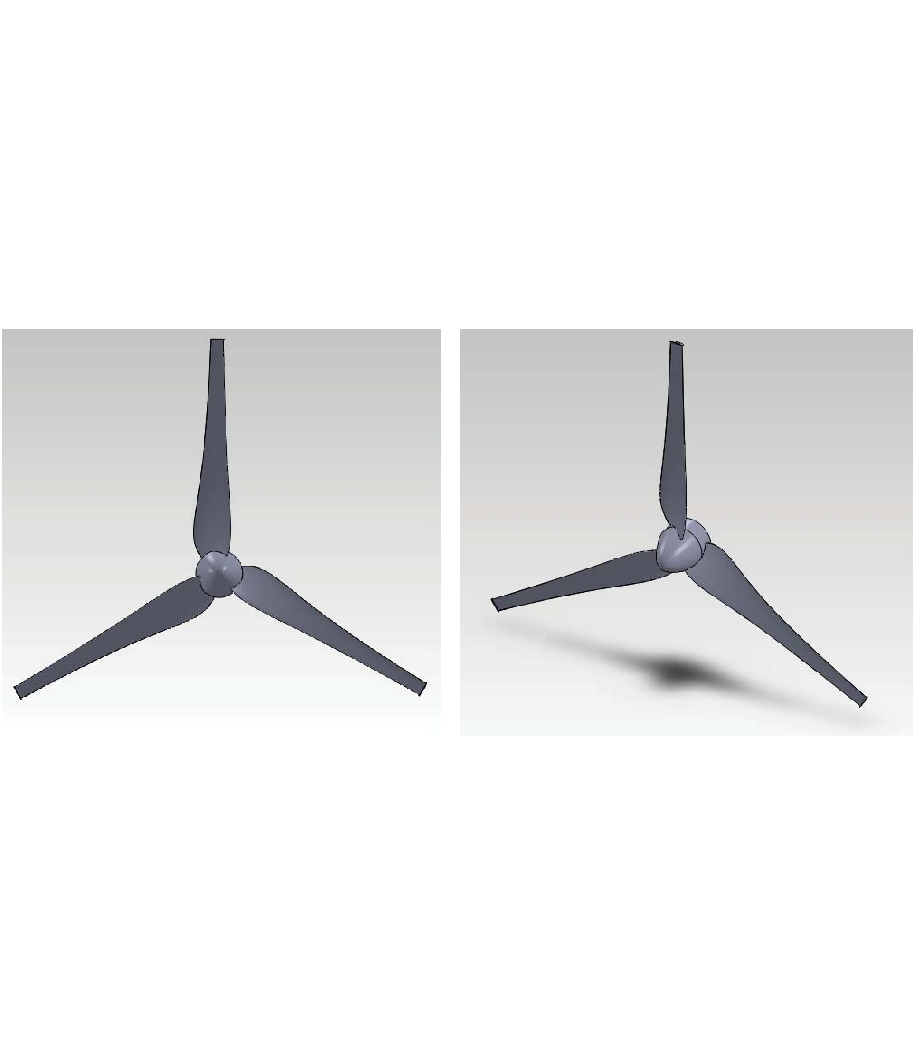
\includegraphics[]{obrazky/celek1}
	\caption{Pohled na celou turbínu}
	\label{cel:1}
\end{figure}
\begin{figure}[H]
	\centering
	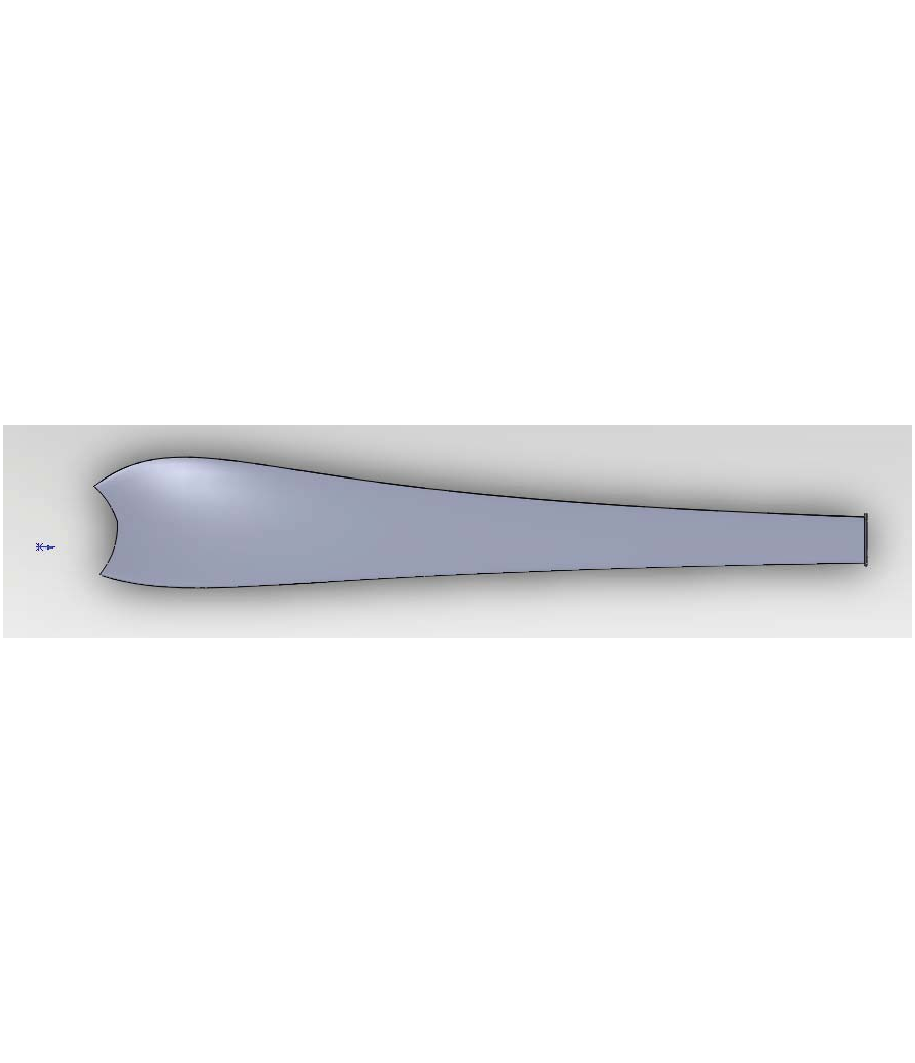
\includegraphics[]{obrazky/celek3}
	\caption{Celkový pohled na list. Modrý bod označuje osu otáčení.}
	\label{cel:2}
\end{figure}
\begin{figure}[H]
	\centering
	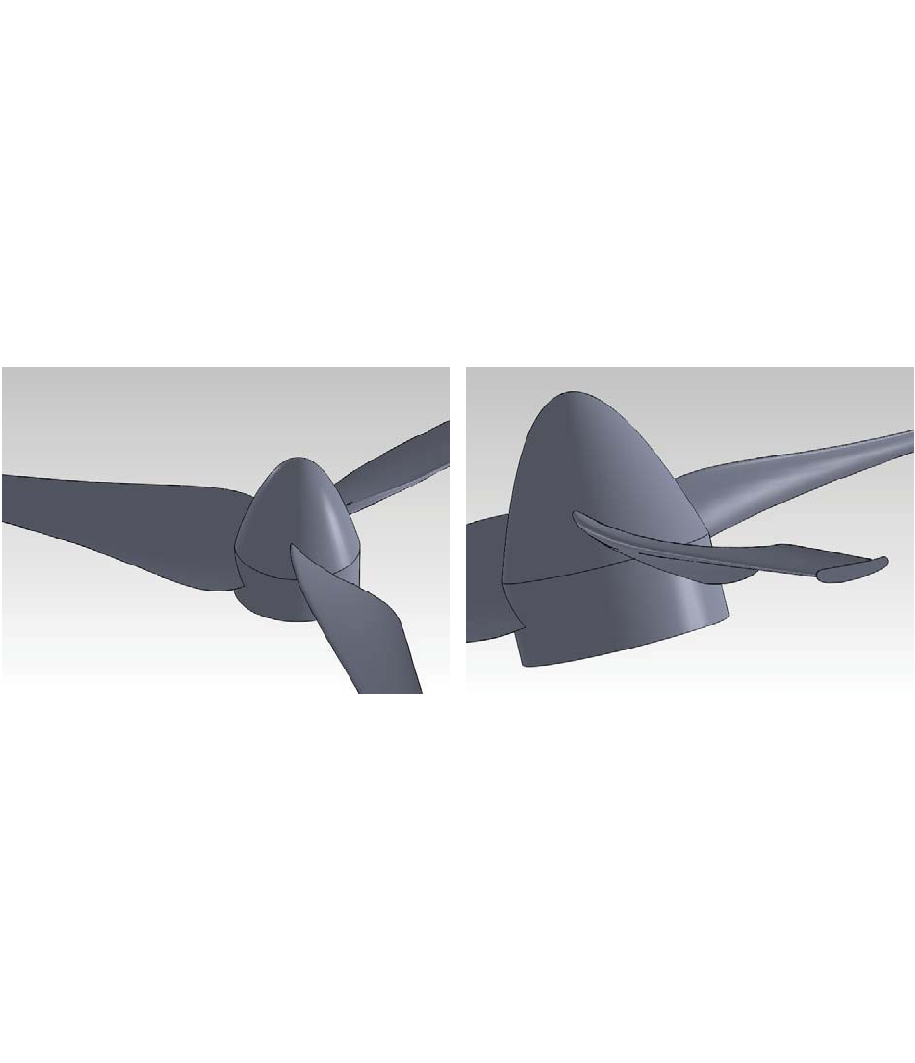
\includegraphics[]{obrazky/celek2}
	\caption{Detail navázání listu na náboj a zakončení listu odsazením}
	\label{cel:3}
\end{figure}
